
\begin{document}

\chapter{Implementation}

\label{chapter:Implementation}

\section{Client}
\label{sec:implementation_client}

The clients and servers communicate through TCP connections. The server opens the a port on the TPC network, and clients request connections to the server via sockets. When a client starts running, it will also start the Kinect. The client will continuously make connection requests until the server responds. If a connection is terminated by the server before the client stops running, the client will keep trying to reconnect to the server.

After the client establishes a connection with the server, it will start sending Kinect Body frames to the server. The low level networking is handled by the Microsoft .Net framework. The client serializes this data before transmitting it to the server, and the server will deserialize it. The server will then passes on the data to the tracker.

\section{Server}
\label{sec:implementation_server}

The application leverages the C\# events and delegates model. The application components subscribe to the event queues of other components. When new data is available from the subscribing component, the subscribed component consumes the data, does something with it, and fires events to all of its subscribed components. The components on the receiving end do the same, and so on. The server assembles the overall communication via events.

The application is started with one parameter, the server port number. It then creates a server to be run at that port number. The server will only start running when it receives such command from the user. After the server is created, it creates the user interface thread as a Single Threaded Apartment running in the background. The user interface will appear now.

The server will receive the following events from the user interface:

\begin{itemize}
  \item Setup parameters for the server
  \item Start the server
  \item Stop the server
  \item When the user interface has displayed the tracking result (then the server will notify the logger)
\end{itemize}

The user will have control over the server, hence the system.

The server will pass the following events to the user interface:

\begin{itemize}
  \item Clients (Kinects) have been connected to the server
  \item Clients (Kinects) have been removed from the server
\end{itemize}

The user interface can know which Kinects are connected to the server, giving the user feedback and later allowing him to choose from which Kinect perspective to view tracked people's skeletons.

The server will bind the following events from the tracker to the user interface:

\begin{itemize}
  \item The tracker is waiting for Kinects to be connected
  \item The tracker is calibrating (and how many frames remaining)
  \item The tracker needs recalibration (and for what reason)
  \item The tracker has synchronized the latest BodyFrame with the tracking result 
\end{itemize}

The user interface would show more feedback, including the latest result, from the tracker.

The application listens for TCP client connections. This work is done in a separate thread, called the ServerWorkerThread. When the TCP socket listener receives a new connection, the server will handle it in a new, separate thread. In the socket thread, the server will create a network stream between the client and the server. After the connection is established, the server will fire a ``OnKinectConnected'' event to the user interface. Later on, the server will receive Kinect BodyFrames from the client through the network stream it had created. Upon receiving some data, the server would deserialize it into a BodyFrame object, then it would fire another event called ``Track'' to the tracker with information about the sender and the BodyFrame itself. Lastly, the server will send a response (a string) back to the client. The response is trivial; it is used to tell the client that the data has been received. The client is also implemented so that it In the current implementation, the server returns ``Okay''. The server will continue to process additional BodyFrames received on its end of the network stream, and the above procedure repeats.

\section{User Interface}
\label{sec:implementation_ui}

The user interface is simplistic (See Figure~\ref{fig:ui}). The researcher has not made the user interface design an important objective due to time constraints. The user interface has a number of buttons for controls on the top. The rest of the user interface below the toolbar is split into halves. The left half, also known as the ``Tracking view'', will visualize the skeletons from the perspective of the reference Kinect. The right half, also known as the ``Disjoined view'', will visualize the skeletons in their original fields of view. Displaying the two different views will demonstrate the current methodology of coordinate transformation. It is worth noting that the 

\begin{figure}[!h]
  \centering

  
\includegraphics[width=0.8\linewidth]{figs/ui}
  
  \caption{The user interface showing the startup screen}
  
  \label{fig:ui}
\end{figure}

The skeleton visualization in both Tracking View and Disjoined View is based on the same implementation. The bones of the skeletons are drawn first, then the joints. The list of human bones consisting of the joints is taken from the Microsoft Kinect Developer examples. The code for the skeleton visualization is also modified based on examples in the official SDK.

The Tracking view shows the average skeleton and the potential skeletons in the same Kinect field of view (See the areas with black backgrounds in Figure~\ref{fig:tracking_disjoined_views}). The average skeletons are in white color, and the potential skeletons of the same person will share the same color. The Disjoined view shows the skeleton visualization of the tracked skeletons in their original Kinect camera space. The skeletons are colored with respect to different Kinects. In other words, skeletons from the same Kinect will share the same color, and skeletons from different Kinects will have different colors.

\begin{figure}[!h]
  \centering
  \subfloat[A person standing in the center of the scene, from the perspective of the Kinect perpendicular to the person]{
    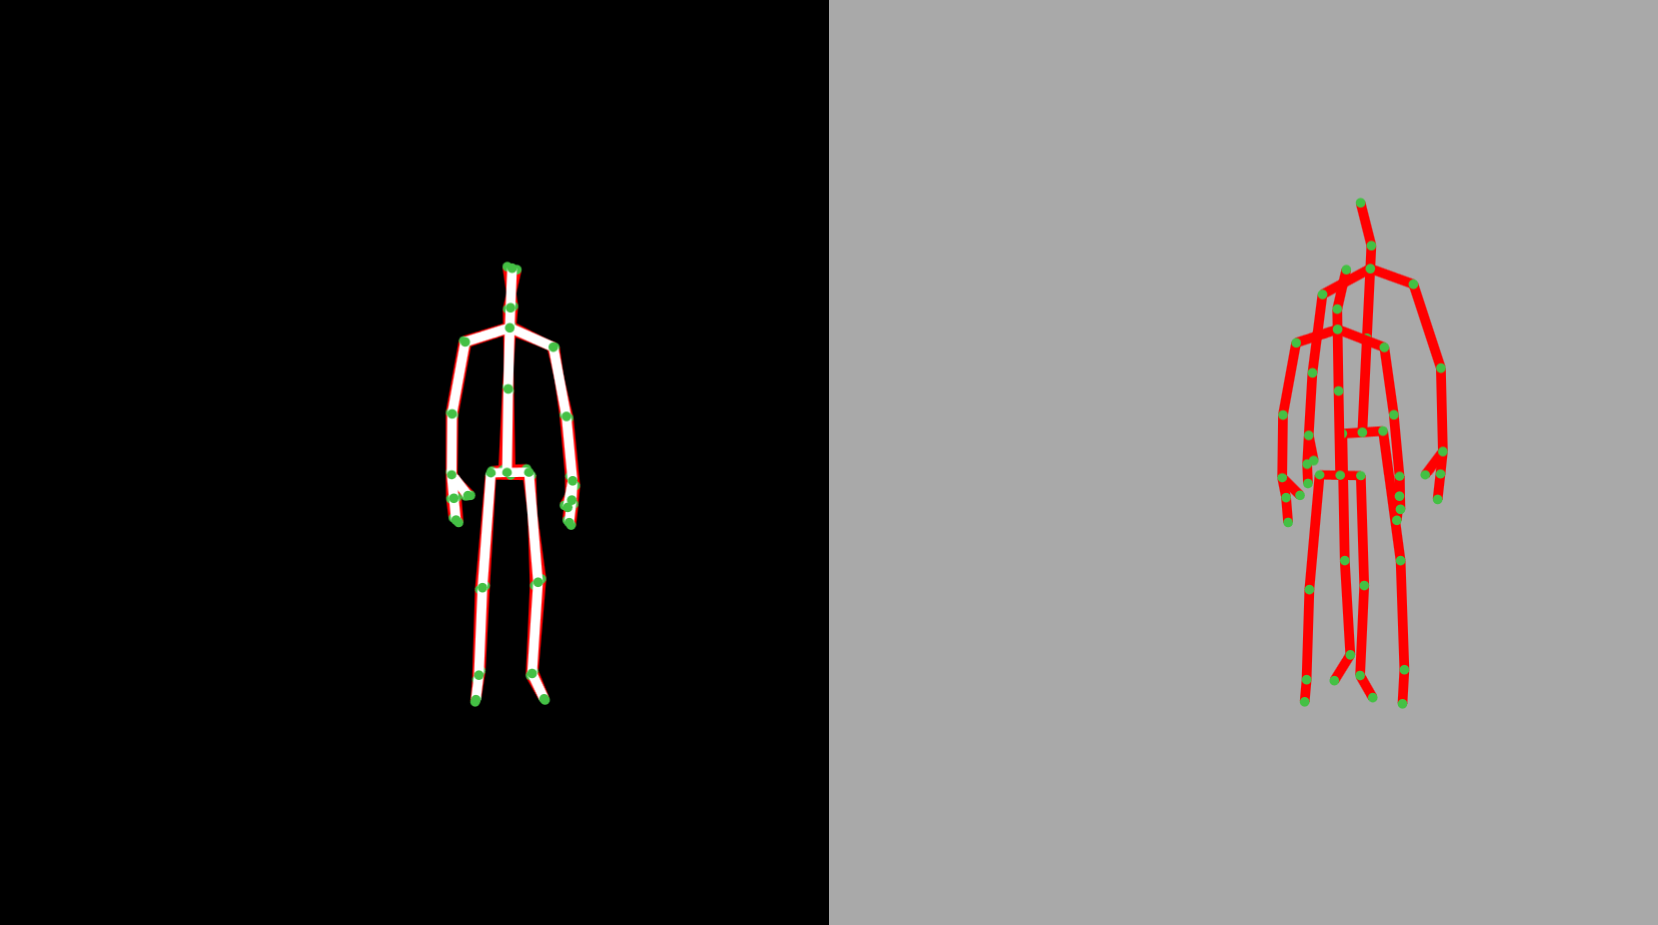
\includegraphics[width=0.5\linewidth]{figs/center_front}
  }
  \subfloat[A person standing in the center the scene, from the perspective of the Kinect at about $45^{\circ}$ from the person]{
    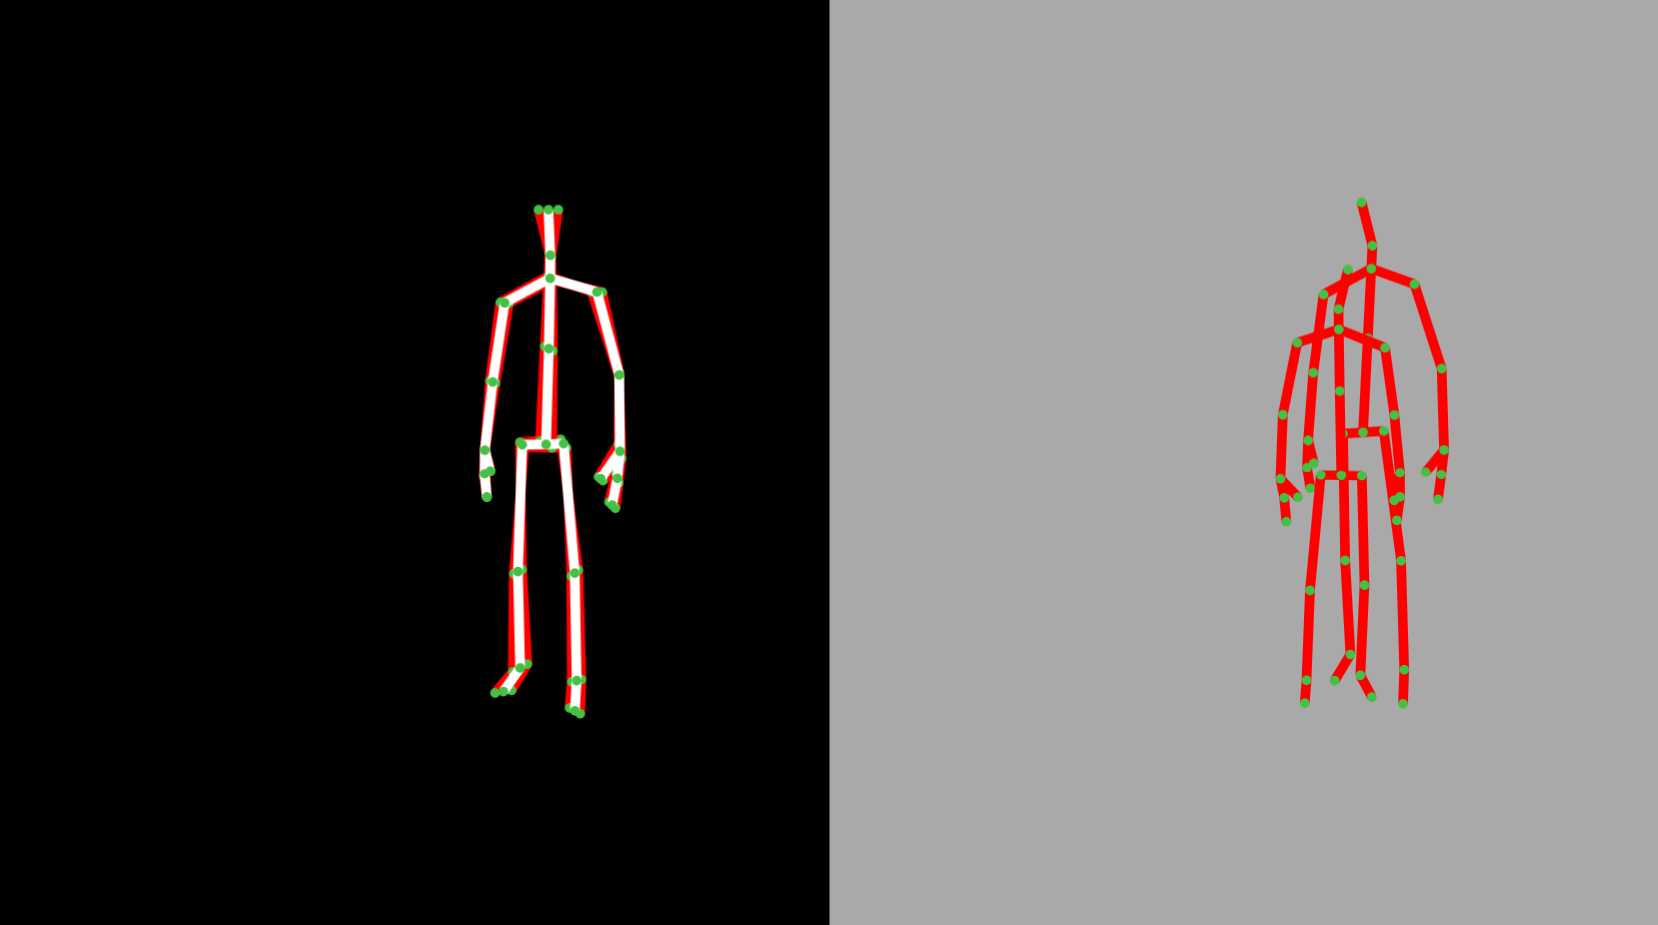
\includegraphics[width=0.5\linewidth]{figs/center_45}
  }
  \\
  \subfloat[A person standing in the back of the scene, from the perspective of the Kinect perpendicular to the person]{
    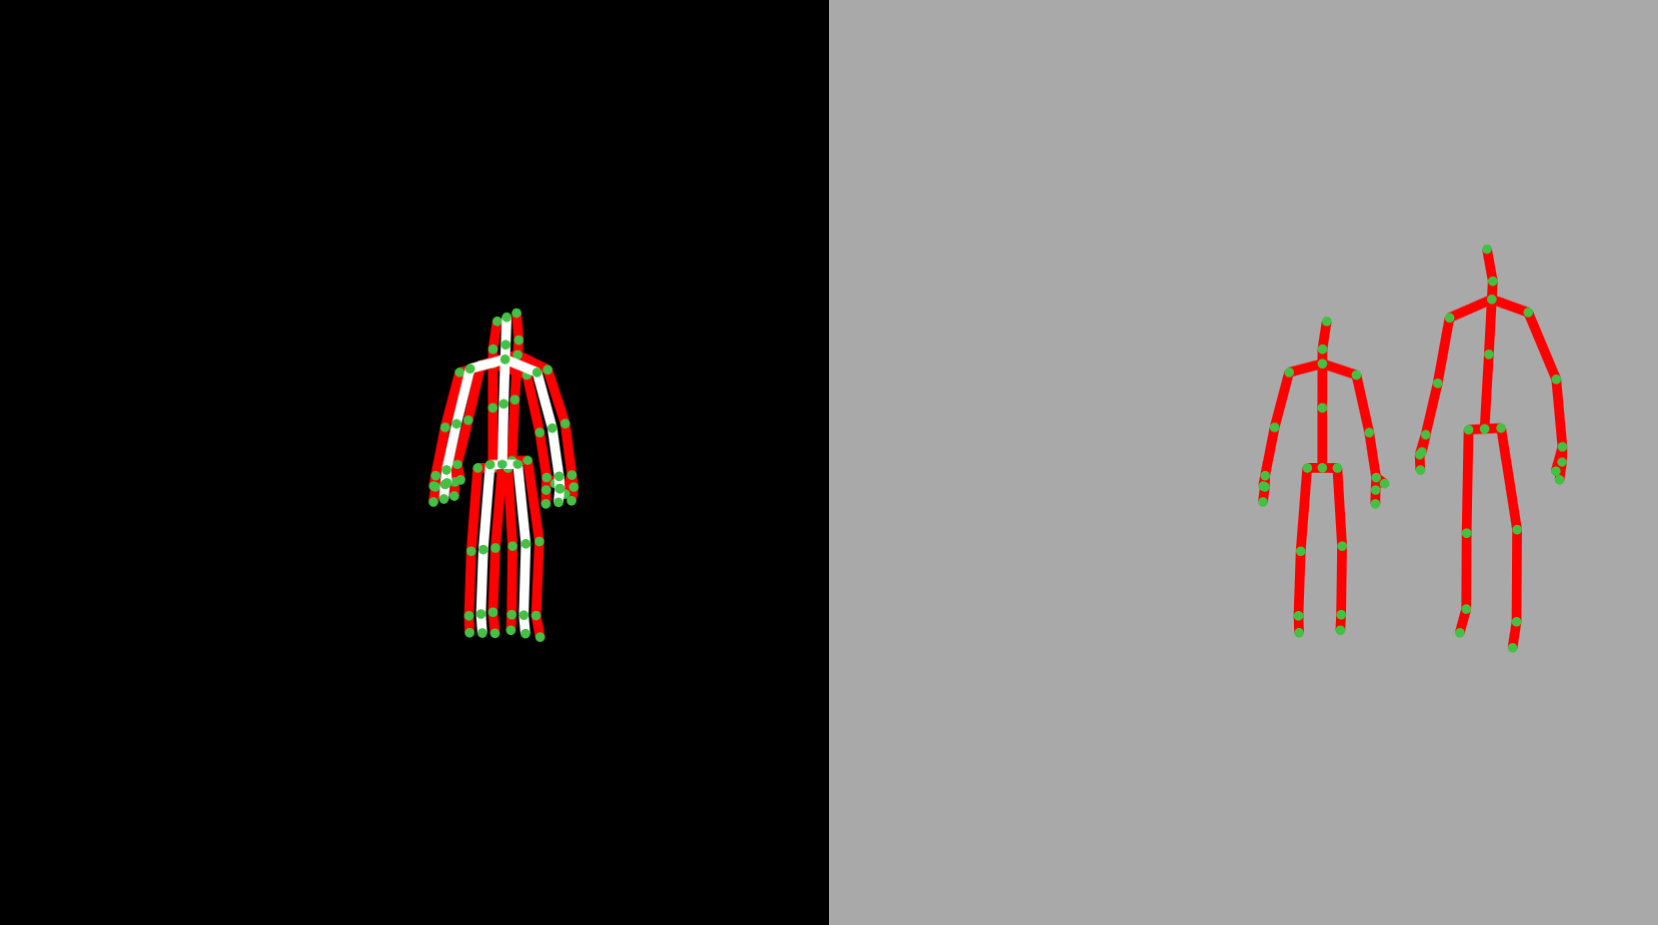
\includegraphics[width=0.5\linewidth]{figs/away_front}
  }
  \subfloat[A person standing in the back of the scene, from the perspective of the Kinect at about $45^{\circ}$ from the person]{
    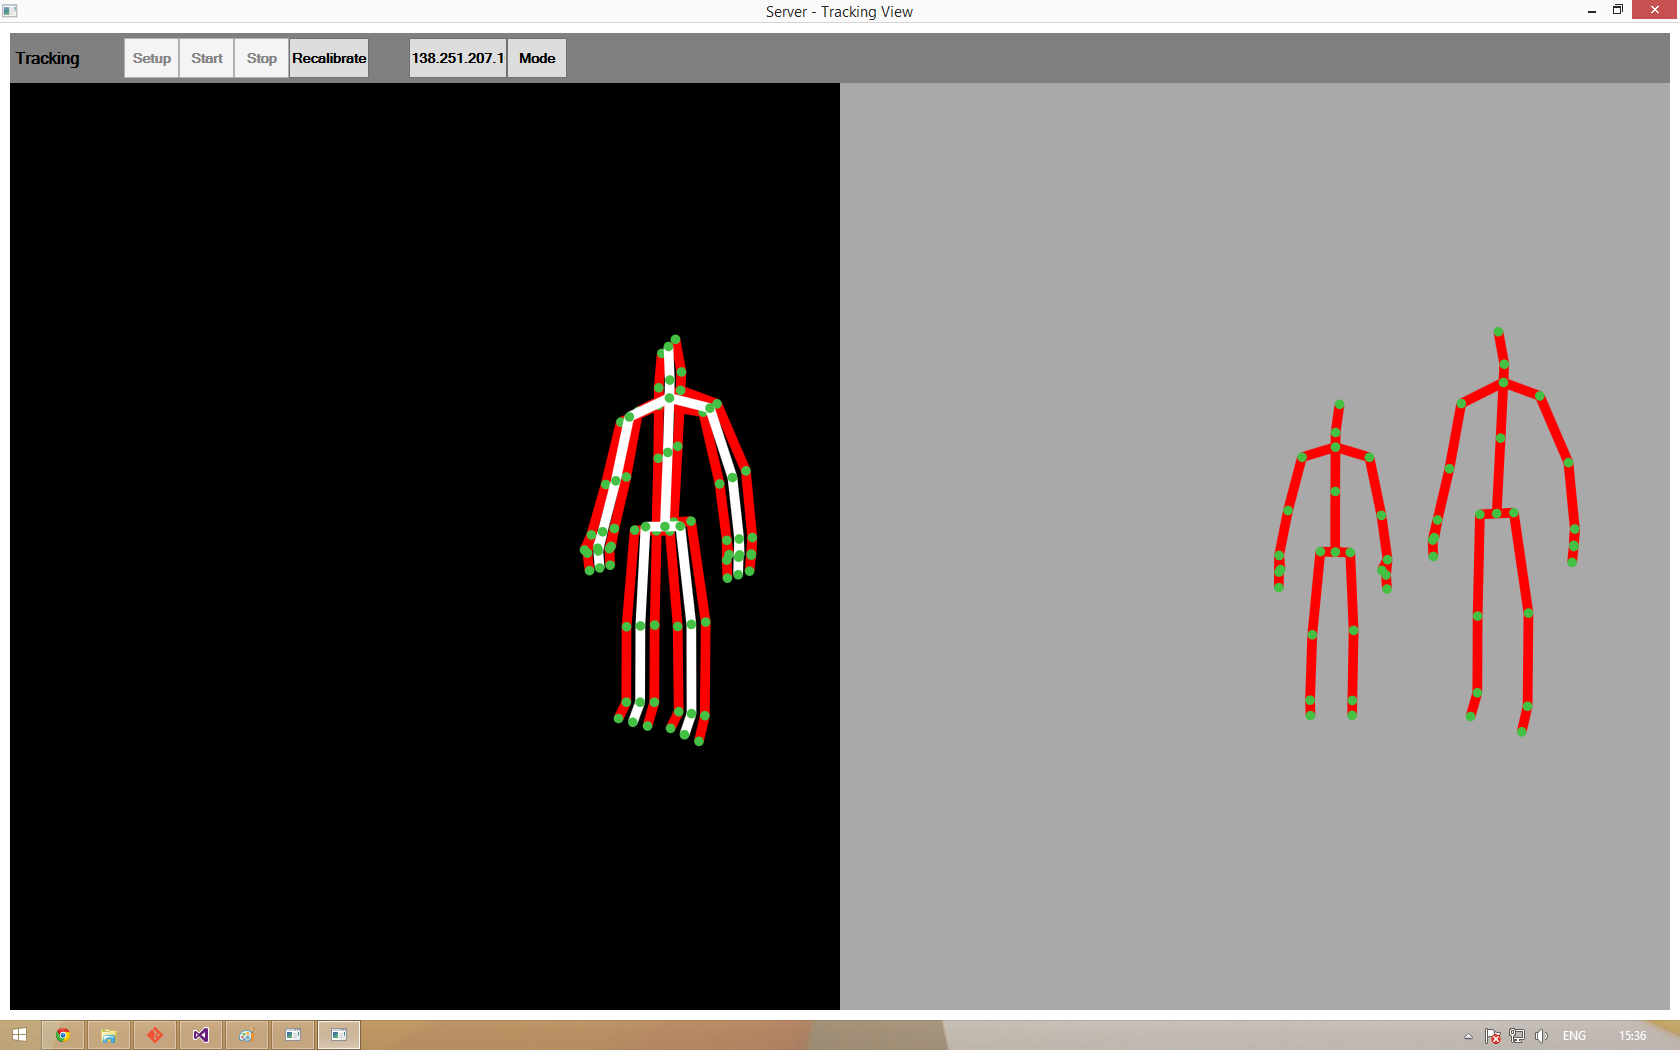
\includegraphics[width=0.5\linewidth]{figs/away_45}
  }

  \caption{The skeleton visualization showing both the Tracking and Disjoined view for for one person standing in different positions and from different perspectives. The areas with a black background are the Tracking views, and the areas with a gray background are Disjoined views.}
  
  \label{fig:tracking_disjoined_views}
\end{figure}

A selection of functionalities are accessible via button clicks. The user interface responds to click events on the buttons. The buttons are disabled when their corresponding functionalities are not available For instance, when the start button is pressed to start the server, the setup button which exposes the configuration of the server will be disabled. When the user interface receives events from the server about client connection and disconnection, the user interface will add or remove the option to transform the current skeletons into the particular Kinect's field of view. The user interface would also display texts in the Tracking view about the progress of calibration or any unexpected behaviour from the user, such as when the user moves during calibration.

\section{Tracker}
\label{sec:implementation_tracker}

The tracker runs the tracking algorithm on the server. Much of the algorithm has been explained in Section~\ref{chapter:current_approach}. This section will explain how the algorithm has been implemented.

The tracker contains a dictionary of clients' IP address (as key) and a generic data structure (as value), called kinectClient, storing information about the Kinect connected to the client and all the frames received from it.

In calibration phase, all frames are stored in a stack inside each KinectClient. This allows the tracker to quickly find the latest 120 frames for calibration. Each KinectClient also keeps track of a list of active skeletons, or TrackingSkeletons. Throughout the lifetime of a tracking process, the tracker updates the position of the TrackingSkeletons.

\section{Logger}
\label{sec:implementation_logger}

The logger takes a tracking result and writes it to the file. The complete list of items logged at each time interval can be found in Appendix~\ref{sec:appendix_logging}.

During the experiments, after the user interface displays the tracking result, it will fire an event to the server. The server will write every other tracking result to a file on the local disk. The user interface will not signal the server about the result if the experiment is paused between tasks.

The logger receives the joint coordinates in World coordinate system (as stored in the result), therefore, it converts them into coordinates in the local Kinect's camera space. The local Kinect is the one which is connected to the server machine via a TCP client. The logger flushes the buffer after it completes the action.

\end{document}
